\documentclass[10pt, a4paper]{article}

\usepackage[paper=a4paper, left=1.5cm, right=1.5cm, bottom=1.5cm, top=3.5cm]{geometry}
\usepackage[utf8]{inputenc}
\usepackage[spanish]{babel}
\usepackage{framed}
\usepackage{endnotes}
\usepackage{graphicx}
\usepackage{multicol}
\usepackage{color}
\usepackage{framed}
\usepackage{xcolor}

\definecolor{gray}{HTML}{E4E6E8}

\newcommand{\notaClase}[1]{\subparagraph{NC.: } {\color{blue}\footnotesize  #1}}
\newcommand{\eg}[1]{ \vspace{0.3cm}
\hspace{0.3cm}
\fcolorbox{black}{gray}{
\begin{minipage}[b]{0.85\textwidth}
\small \textsf{
#1 
}
\end{minipage}
}
}

\renewcommand\notesname{Notas Finales}

%Datos para la caratula
\title{Exokernel \\ \small{Apuntes de presentación}}

\author{E. Mancuso - A. Mataloni - M. Miguel}

\date{16 de Junio de 2011}

\begin{document}

\maketitle

\section{Introducción}

\subsection{Análisis del problema}
El concepto de Exokernel es una propuesta para una nueva filosofía en la confección de kernels. Esta propuesta está motivada por las siguientes observaciones:

Los kernels de hoy en día...
\begin{itemize}
 \item ... son poco flexibles.
 \item ... día deben dar soporte a una gran variedad de tipo de aplicaciones.
 \item ... pierden eficiencia en la generalidad y el grosor de trabajo que deben hacer.
\end{itemize}

Los kernels monolíticos fuerzan ciertas implementaciones de distintas abstracciones de alto nivel como procesos, archivos e IPC, y ocultan información de lo que sucede en el hardware que está debajo. En el esquema actual, las aplicaciones corren en máquinas virtuales que están provistas de todas estas abstracciones. Todo esto produce cierta inercia en el desarrollo de sistemas operativos que evita innovación en la implementación de las abstracciones y además no permite a las aplicaciones beneficiarse del uso del hardware. Además, en la generalidad de aplicaciones que los kernels intentan soportar, obligan a las mismas a pagar costos en su performance por utilidades que le son provistas pero no utiliza. 

\eg{En muchos casos las aplicaciones deben emular componentes de hardware que les fueron ocultados, como ser las bibliotecas de multithreading que emulan las interrupciones del timer-tick. Otro ejemplo son las bases de datos que deben emular acceso aleatorio por encima de los filesystems.} 

\eg{Además, \emph{garbage collectors} y bases de datos relacionales pueden beneficiarse enormemente por una mejor relación con el manejo del Hardware ya que, por ejemplo, poseen accesos de datos predecibles. Sería una gran mejora utilizar esta información a la hora de desalojar páginas.}

\subsection{Presentación de la solución}
Frente a estas inquietudes es que se plantea el concepto del Exokernel. Un exokernel es un kernel minimal que multiplexa los servicios de hardware de modo seguro. Exporta el hardware en lugar de emularlo. Lo que se está haciendo es separar la protección de los recursos de su administración, encargándose solo de la primera. Esto último está inspirado por la observación de que \emph{cuanto más bajo es el nivel de abstracción de una función primitiva, más eficientemente puede ser esta implementada}. Luego, todas las abstracciones de los sistemas operativos son implementadas en el nivel de las aplicaciones. Esta es la filosofía que se plantea para generar ambientes más flexibles y darle mayor participación a las aplicaciones en la administración de sus propios recursos. 

\begin{figure}[H]
\centering
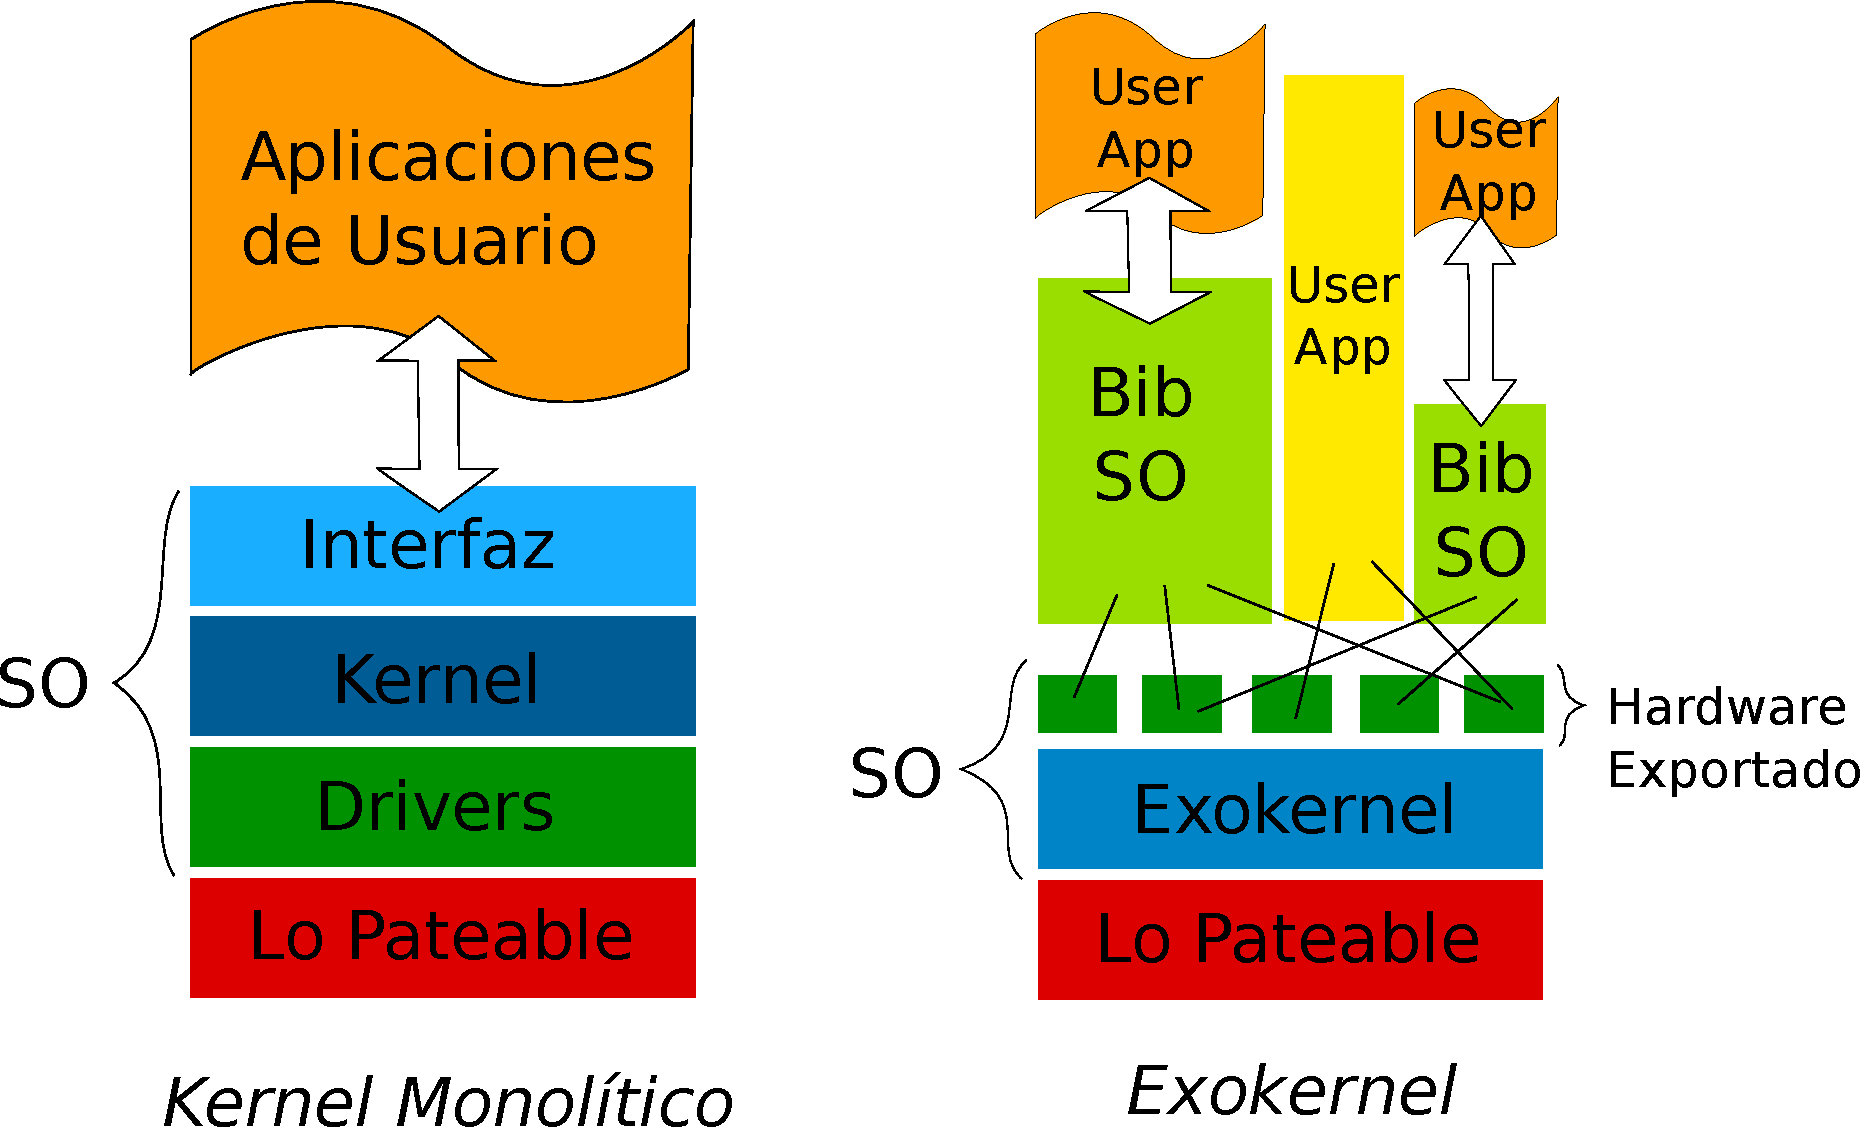
\includegraphics[scale=0.5]{grafico-kernel-exokernel.pdf}
\caption{Gráfico comparativo de los módulos en un kernel monolítico y un exokernel}
\end{figure}

El gráfico superior muestra una comparación en la arquitectura de un kernel monolítico y un exokernel. En el primero, la pila de módulos de desarrolla en una única línea vertical. El kernel exporta una única interfaz que es utilizada por todas las aplicaciones de usuario. En un exokernel, el hardware se exporta para ser utilizado de variadas formas. En el ámbito del exokernel, se habla de \emph{bibliotecas de sistema operativo}, como un módulo que implementa las abstracciones clásicas de los sistemas operativos (espacios de direcciones, IPC, procesos, archivos, etc.), sobre los cuales pueden ejecutarse aplicaciones de la forma clásica. Estas implementaciones se hacen en el nivel de aplicación. El punto importante es que, como muestra el gráfico, el exokernel permite la convivencia de varias \emph{bibliotecas de sistemas operativos} que utilizan distintas abstracciones o implementaciones de las mismas y las aplicaciones de usuario pueden elegir aquellas que les resulten más conveniente para su performance. A su vez, en este esquema, las aplicaciones pueden elegir manejar recursos de hardware por si mismas para lograr mejores resultados. 

El concepto de exokernel se maneja por las siguientes filosofías:

\begin{itemize}
 \item Las aplicaciones saben mejor que el sistema operativo cuál es su objetivo y como manejar sus recursos, por lo que deberían tener tanto control de estos como sea posible. 
 \item Cuanto más bajo es el nivel de abstracción de una función primitiva, más eficientemente puede ser esta implementada y es más fácil verificarla y potabilizada. 
\end{itemize}


\end{document}